\chapter{Théorie d'un réseau acoustique fini constitué de résonateurs de Helmholtz}
Ce chapitre a pour but de caractériser le champ de pression dans un guide sur lequel des résonateurs de Helmholtz sont placés en dérivation, espacés régulièrement d'une longueur $L$. On dispose pour cela d'un banc de mesure représenté en figure ~\ref{schema_infini}. Une simulation de la propagation dans le réseau pourra donc être confronté à une expérience.

\begin{figure}[!ht] \centering
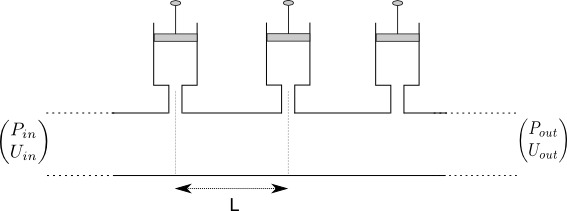
\includegraphics[scale=0.5]{./images_chp1/schema_reseau_infini.png}
\caption{\label{schema_infini} Schéma du réseau de résonateurs de Helmholtz.}
\end{figure}

\paragraph{Notations}
Le guide principal a pour section $S$ ; le col des résonateurs a pour longueur $L_{n}$ et pour section $S_{n}$ ; la cavité des résonateurs a pour longueur $L_{c}$ et pour section $S_{c}$. Par la suite, on note $\rho$ la masse volumique de l'air et $c$ la célérité du son dans l'air.

\section{Mise sous forme matricielle}
On s’intéresse ici a la mise sous forme matricielle du problème de la propagation acoustique dans le réseau periodique vu ci-dessus. Le but est de mettre en relation les pressions et débits en entrée du système ($P_{in}$ et $U_{in}$) avec ceux en sortie ($P_{out}$ et $U_{out}$) sous la forme suivante:
\begin{equation}
\begin{pmatrix} P_{out} \\ U_{out} \end{pmatrix} =\begin{pmatrix} a & b \\ c & d \end{pmatrix}^N \begin{pmatrix} P_{in} \\ U_{in} \end{pmatrix} = \begin{pmatrix} A & B \\ C & D \end{pmatrix} \begin{pmatrix} P_{in} \\ U_{in} \end{pmatrix} .
\end{equation}

Cette matrice dispose en effet de propriétés intéressantes et l'étude du système sera grandement facilité par ce formalise. De plus, les simulations sont faciles à mettre en œuvre dès lors que celle ci est connue.

Pour cela, les 2 éléments du réseau (guide et résonateur) doivent être mis sous forme matricielle puis multipliés.

\subsection{Le guide d'onde}
Le problème est considéré à une dimensions du fait de la longueur du guide et du domaine de fréquence de l'étude: on considère que seul des ondes planes se propagent.
La solution de la propagation dans un guide d'onde peux être facilement déduite de l'équation d'onde suivante :
\begin{equation}
\frac{\partial ^2 p}{\partial x^2} -\frac{1}{c^{2}} \frac{\partial ^2 p}{\partial t^2}= 0
\end{equation}
On se place en régime harmonique et on note $\Gamma = jk$ la constante de propagation du système. D’où les solutions (vitesses calculées avec l'équation d'Euler:

\begin{eqnarray*}
\begin{cases}
p(x_1)  =  C_1 e^{-\Gamma x_1} + C_2 e^{\Gamma x_1} \\
v(x_1)  =  -\frac{1}{j\omega\rho} [ -\Gamma C_1 e^{-\Gamma x_1} + \Gamma e^{\Gamma x_1}]\\
p(x_2)  =  C_1 e^{-\Gamma x_2} + C_2 e^{\Gamma x_2} \\
v(x_2)  =  -\frac{1}{j\omega\rho} [ -\Gamma C_1 e^{-\Gamma x_2} + \Gamma e^{\Gamma x_2}]
\end{cases}
\end{eqnarray*}
 
On pose $x_1 - x_2 = L$. Tous calculs faits, on trouve finalement:
\begin{eqnarray*}
\begin{pmatrix} p(x_1) \\ v(x_1) \end{pmatrix} = \begin{pmatrix} \cosh(kL) & \frac{j\omega\rho}{k} \sinh(k L) \\  \frac{k}{j\omega\rho}\sinh(k L) & \cosh(k L) \end{pmatrix} \begin{pmatrix} p(x_2) \\ v(x_2) \end{pmatrix}
\end{eqnarray*}

La première fréquence de coupure du guide est donc d'environ $4kHz$ pour les dimensions du réseau que nous considérons. Dans la suite, on supposera donc que seul le mode plan est propagatif. Les simulations et mesures ne seront donc faite que sur une bande de fréquences allant de $0$ à $1~kHz$.

\subsubsection{Ajout des pertes}
\todo[inline]{source biblio à citer}

Pour prendre en compte les pertes, on modifie l'expression de la constante de propagation et de l'impédance caractéristique. Les expressions sont donc:
\begin{eqnarray*}
 k =  \frac{\omega}{c_0} \left( 1 + \frac{\beta}{s}(1+(\gamma-1)/ \chi \right) \\
 Z_c =  \frac{\rho c_0}{S} \left( 1 + \frac{\beta}{s}(1-(\gamma-1)/ \chi \right) 
\end{eqnarray*}

Dans ces expressions, on a:
\begin{itemize}
 \item  $s=R/ \delta$ avec $\delta = \sqrt{\frac{2 \mu}{\rho \omega}}$
 \item  $\chi = \sqrt{P_r}$ ou $P_r$ est le nombre de Prandtl
 \item $\beta = (1-j)/\sqrt{2}$ 
 \item $\mu$ la viscosité de l'air
\end{itemize}

Du fait de la géométrie assez complexe du système, ces pertes ne peuvent pas être négligées comme cela peux être souvent le cas en acoustique.

\subsection{Impédance d'entrée d'un résonateur}
Le résonateur de Helmholtz est considéré dans le réseau comme un changement ponctuel d'impédance. Cette impédance, notée $Z_{r}$ peut être calculée en utilisant le même formalisme matriciel que précédemment.



 %Cette impédance peux être calculée via la formule de l'impédance ramenée ~\ref{imp_ramenee}. De plus, les dimensions utilisées dans la suite sont corrigées afin de prendre en compte les corrections de longueurs liés à la géométrie du problèmes. Ces formules de corrections sont disponibles en annexe 2.
%\begin{eqnarray}
%Z{x_1}=\frac{jZ_c tan(kL)+Z_{x_2}}{1+j\frac{Z_{x_2}}{Z_c}tan(kL)}.
%\label{imp_ramenee}
%\end{eqnarray}

On suppose que le résonateur est constitué de 2 guides à parois rigides d'impédance caractéristique $Z_{n}=\rho c/S_{n}$ pour le col et $Z_{c}=\rho c /S_{c}$ pour la cavité. La matrice de transfert mettant en relation les pression et débit à l'entrée du résonateur $P_e$ et $U_e$ et les pression et débit au niveau de la paroi extrême $P_s$ et $U_s=0$ est de la forme :
\begin{eqnarray*}
\begin{pmatrix} P_e \\U_e \end{pmatrix} & = & \begin{pmatrix} \cos(k L_n) & j Z_{n} \sin(k L_n) \\ \frac{1}{Z_{n}} \sin(k L_n) & \cos(k L_n) \end{pmatrix} \begin{pmatrix} \cos(k L_c) & j Z_{c} \sin(k L_c) \\ \frac{1}{Z_{c}} \sin(k L_c) & \cos(k L_c) \end{pmatrix} \begin{pmatrix} P_s \\ 0  \end{pmatrix} \\
\begin{pmatrix} P_e \\U_e \end{pmatrix} & = & \begin{pmatrix} r_1 & r_2 \\ r_3 & r_4 \end{pmatrix} \begin{pmatrix} P_1 \\ 0  \end{pmatrix} \\
~ & \Rightarrow & Z_{r}	 = \frac{P_e}{U_e}= \frac{r_1}{r_3}
\end{eqnarray*}

\paragraph{Correction de longueur}
La longueur effective du col est sujet à une correction présentée en annexe \ref{annexe_corr}.

En ajoutant un résonateur en parallèle au guide, il y a toujours continuité des pressions mais plus des vitesses. La matrice de transfert pression-débit pour un résonateur dans le réseau est alors la suivante :

\begin{eqnarray*}
M_{r} = \begin{pmatrix} 1 &  0 \\ 1 /Z_{r} & 1  \end{pmatrix}\\
\end{eqnarray*}

\section{Étude du réseau fini}

Une fois les matrices de guide et de résonateur connues, il suffit alors de les multiplier afin d'obtenir la matrice d'une cellule du réseau. C'est sur l'étude de cette matrice que se basent les analyses de cette section. 

Dans la suite les paramètres de la simulation sont ceux de l'expérience dont nous disposons. Ces paramètres sont disponible en annexe 2.

\subsection{Équation de dispersion}
La matrice de transfert l'équation de dispersion pour le réseau à N cellules s'écrit alors : 
\begin{equation}
\cos(NkL) = \frac{A+D}{2} 
\end{equation}

Ainsi, on peut remonter à une expression de $kL$ en fonction de la fréquence. En particulier, les zones où $kL$ devient imaginaire nous intéressent particulièrement car cela induit une décroissance exponentielle de l'onde de propageant dans le guilde (onde évanescente). Ces bandes sont appelées les bandes de Bragg.

\subsection{Réflexion et transmission du réseau}
Le coefficient de réflexion et de transmission du réseau complet peut être calculé de la manière suivante [\todo[inline]{Source biblio}] : 
\begin{eqnarray}
T & = & \frac{2}{A + B/Z_c + C Z_c + D} \\
R & = & \frac{A + B / Zc_ - C Z_c -D}{A + B/Z_c + C Z_c + D} 
\end{eqnarray}

On trace ces coefficients en fonction de la fréquence (figure~\ref{ex_coef_RT}) ainsi que l'admittance des résonateurs utilisés. Il apparaît que la transmission chute pour trois bandes de fréquence : à la résonance du résonateur de Helmholtz, à celle de sa cavité et à la première bande de Bragg.

\subsection{Bande de Bragg}
Ces bandes sont visibles dès que des singularités apparaissent de manière periodique. L'énergie de l'onde est reste contenue entre chaque éléments du fait que la longueur d'onde correspond à la moitié de l'espacement entre 2 éléments. 

Pour un espacement entre éléments de longueur $L=0.1~m$, la bande de Bragg se situe autour de la fréquence $f_{b} = \frac{c}{2L} = 1715 Hz$. On constate sur la figure~\ref{ex_coef_RT} que ces bandes de Bragg sont bien présentes à la fréquence indiquée ainsi qu'a ses multiples (chute de la transmission et réflexion maximale).
 

\subsection{Bande interdites liés aux résonateurs}
L'équation de dispersion est cependant plus difficile à analyser qu'il n'y parait en raison des résonateurs qui constituent réseau. Ceux-ci ont une impédance négligeable dès lors que la fréquence d'analyse se trouve suffisamment éloigné des fréquences de résonances. 

De plus le résonateur étant par nature un système résonant, il peut lui aussi induire une absorption de l'énergie de l'onde sur certaines fréquences. Sur la figure~\ref{ex_coef_RT}, ces bandes interdites sont aussi présentes: elles se trouvent là ou l'admittance du résonateur est maximale. A ces fréquences, on a bien une chute de la transmission.

\begin{figure}
\centering
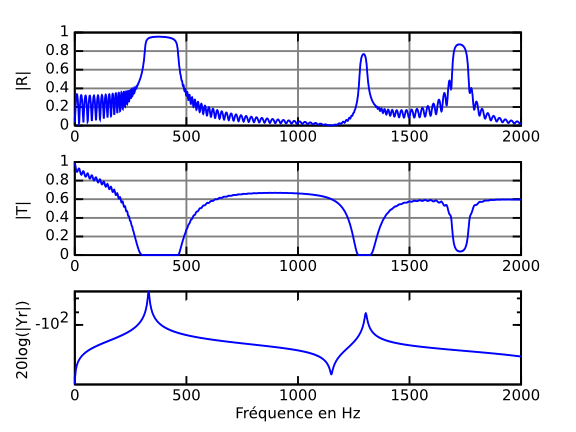
\includegraphics[scale=0.7]{./images_chp1/ex_coef_rapport.png}
\caption{\label{ex_coef_RT} Coefficient de réflexion (en haut) et de transmission (au milieu) pour un réseau de 60 résonateurs avec $L_c=14~cm$. En bas : Impédance d'entrée du résonateur.}
\end{figure}

\subsection{Cas désordonné}

\subsubsection{Désordre sur le volume des cavités}

Afin d'étudier succinctement l'effet d'un désordre sur le volume des cavités du résonateur, une simulation numérique est réalisée pour des longueurs de cavité suivant une loi normale. Comme précédemment, les résonateurs sont arbitrairement au nombre de 60 et sont séparés d'une distance $L=0.1$ m. La figure~\ref{chaos10} présente les coefficients de transmission et de réflexion pour une longueur de cavité moyenne de $\bar{L_c}=14$ cm et un écart-type  de $\sigma = 1$ cm.


Dans le cas d'un écart-type élevé, le désordre a pour principal effet d'élargir la bande interdite liée à la seconde résonance des résonateurs (résonance de la cavité). La bande de Bragg n'est pas impactée puisque le désordre touche le volume des cavités et non l'espacement des résonateurs.

\paragraph{Désordre lié aux conditions expérimentales}
Dans l'expérience menée plus loin, le volume des résonateur est fixé manuellement. La question de l'impact de l'erreur commise par la mise en place de l'expérience est donc directement liée à l'étude de désordre dans le réseau. On estime que la longueur des cavités va suivre une loi normale d'écart-type 2 mm et de longueur moyenne $\bar{L_c}=14$ cm. La figure~\ref{chaos2} montre alors que ce désordre n'a qu'une faible influence sur le coefficient de réflexion. 


\begin{figure}[!h]
	\begin{minipage}{0.45 \textwidth}
		\centering
		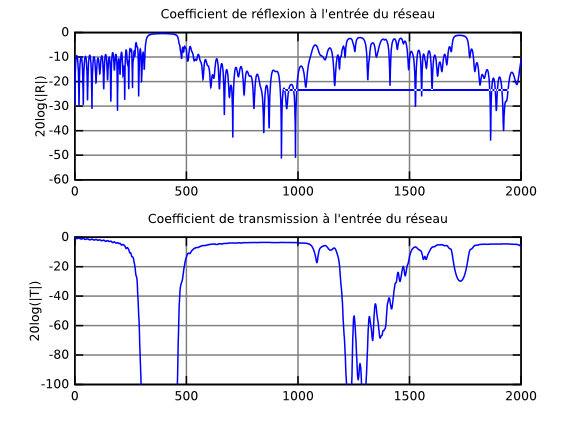
\includegraphics[scale=0.5]{./images_chp1/chaos_10mm.png}
		\caption{\label{chaos10} Coefficient de réflexion (en haut) et de transmission (en bas) pour un réseau de 60 résonateurs avec $\bar{L_c}=14$~cm et $\sigma =1$ cm.}
	\end{minipage}
\hspace{0.5cm}
	\begin{minipage}{0.45 \textwidth}
		\centering
		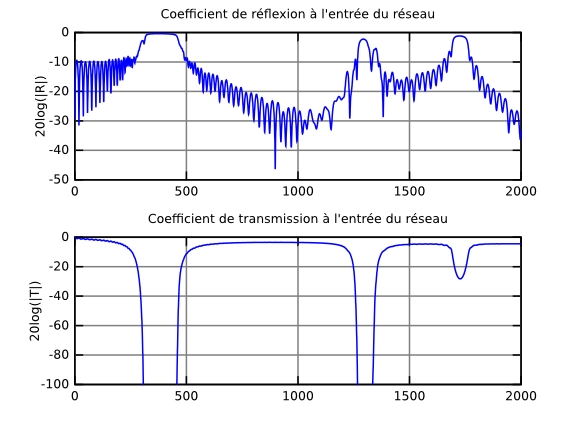
\includegraphics[scale=0.5]{./images_chp1/chaos_2mm.png}
		\caption{\label{chaos2} Coefficient de réflexion (en haut) et de transmission (en bas) pour un réseau de 60 résonateurs avec $\bar{L_c}=14$~cm et $\sigma=2$ mm.}
	\end{minipage}
\end{figure}



\subsubsection{Désordre sur la position des résonateurs}
La même étude est menée sur le désordre lié à la conception du banc de mesure et aux défauts de position des résonateur. La configuration du réseau est la même.
Les figures~\ref{chaospos10} et~\ref{chaospos2} montrent l'effet d'un désordre plus ou moins grand sur la réflexion et la transmission.

\begin{figure}[h!]
	\subfigure[\label{chaospos10}$\sigma=1$ cm]{
		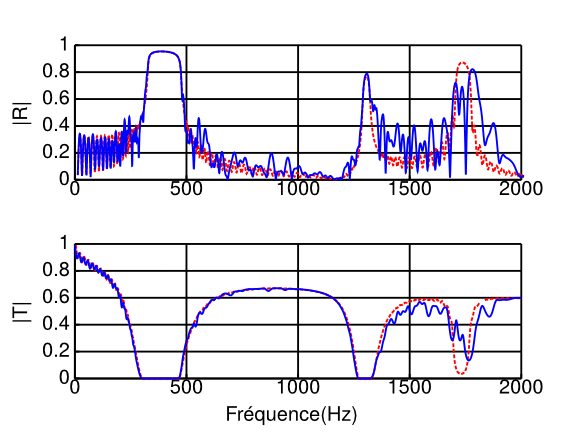
\includegraphics[scale=0.5]{./images_chp1/chaos_position_grand.png}
	}
	\subfigure[\label{chaospos2}$\sigma=2$ mm]{
		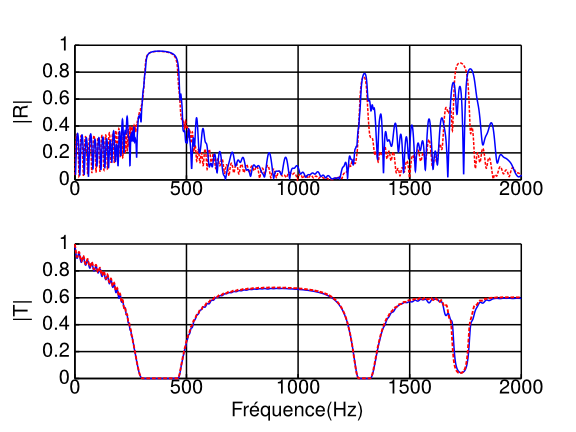
\includegraphics[scale=0.5]{./images_chp1/chaos_position_petit.png}
	}
	\caption{Coefficients de réflexion (en haut) et de transmission (en bas) pour un réseau de 60 résonateurs avec $\bar{L}=14$ cm.}
\end{figure}

Le désordre a pour principal effet d'augmenter la transmission au niveau de la bande de Bragg. Pour un désordre grand, l'effet du réseau n'est plus visible, puisque la bande interdite de Bragg va jusqu'à disparaître.

Le désordre d'écart-type 2 mm est supérieur à celui estimé pour la réalisation du banc de mesure et est cependant moindre. On considère donc qu'il est négligeable par la suite.



